\documentclass{article}


% if you need to pass options to natbib, use, e.g.:
%     \PassOptionsToPackage{numbers, compress}{natbib}
% before loading neurips_2024


% ready for submission
\usepackage{neurips_2024}


% to compile a preprint version, e.g., for submission to arXiv, add add the
% [preprint] option:
%     \usepackage[preprint]{neurips_2024}


% to compile a camera-ready version, add the [final] option, e.g.:
%     \usepackage[final]{neurips_2024}


% to avoid loading the natbib package, add option nonatbib:
%    \usepackage[nonatbib]{neurips_2024}

\usepackage{graphicx} 
\usepackage[utf8]{inputenc} % allow utf-8 input
\usepackage[T1]{fontenc}    % use 8-bit T1 fonts
\usepackage{hyperref}       % hyperlinks
\usepackage{url}            % simple URL typesetting
\usepackage{booktabs}       % professional-quality tables
\usepackage{amsfonts}       % blackboard math symbols
\usepackage{nicefrac}       % compact symbols for 1/2, etc.
\usepackage{microtype}      % microtypography
\usepackage{xcolor}         % colors

\usepackage{biblatex} %Imports biblatex package
\addbibresource{bibliography.bib} %Import the bibliography file

\title{Semiconductor Layout Design with Large Language Models: Opportunities and Challenges}

\author{%
  Bo Wen\\
  IBM Watson Research Center, \\
  Yorktown Heights, NY, USA \\
  \texttt{bwen@us.ibm.com} \\
  \And
  Xin Zhang\\
  IBM Watson Research Center, \\
  Yorktown Heights, NY, USA \\
  \texttt{xzhang@us.ibm.com} \\
}

\begin{document}

\maketitle

\begin{abstract}
  % Update abstract to reflect the content of the paper
  This paper explores the potential of large language models (LLMs) as a "layout design copilot" in various domains such as semiconductor, IC, and microfluidics. We evaluate the capabilities of LLMs in generating basic elements and combining them into complex designs. Our experiments focus on via connections, microfluidics channel design, and fiducial marker generation. We discuss the opportunities and challenges of using LLMs in layout design, highlighting the importance of providing expert knowledge and context to improve their performance.
\end{abstract}

\section{Introduction}
% Brief overview of layout design in various domains
% Challenges in automating repetitive tasks while maintaining flexibility 
% Potential of large language models (LLMs) as a "layout design copilot"
% Thesis statement and paper overview

\section{Methodology}
\subsection{Basic Element Generation}
% Evaluation of popular LLMs in drawing basic shapes (zero-shot attempt)
% Suggestion: Present a table showcasing success rates
% Conclusion: Setting up a RAG system with working example code improves accuracy

A total of 25 examples were generated using ChatGPT-4o, Python code was generated to write a GDSII files for the desired elements, accompanied by human evaluation. In instances where the model did not produce the correct output on the first attempt, a researcher would provide step-by-step guidance until achieving the desired result. However, in the case of generating a serpentine pattern, the model encountered difficulties, likely due to an unfamiliarity with the \texttt{gdspy.FlexPath} function. To address this, an example code was provided to the model, enabling it to 'learn' and successfully generate the correct serpentine sample file.

\subsection{Combining Basic Elements into Complicated Designs}
% Introduction to the three explored use cases
\paragraph{Via connection in semiconductor process}
\paragraph{Microfluidics channel design}


\section{Results and Discussion}
\subsection{Via Connection Experiment}
\subsubsection{Background}
In semiconductor processes, vias are essential for creating electrical connections between different layers of a chip. Proper via placement and connection are crucial for ensuring the functionality and reliability of the integrated circuit. This experiment explores the potential of using large language models (LLMs) to generate layout designs for via connections based on natural language descriptions and color-coded sketches.
\subsubsection{Experimental Setup}
The sketch-to-design approach using LLMs involves providing a natural language description of the desired via connection layout along with a color-coded sketch. The input format consists of a text description specifying the layers, dimensions, positions, and connectivity requirements, as well as a corresponding sketch where each color represents a specific layer (e.g., yellow for via, blue for metal, red for pad). The target output is Python code that generates the GDSII layout based on the provided description and sketch.
\subsubsection{Iterative Testing and Results}
We conducted a series of tests to evaluate the LLM's performance in generating via connection layouts. Figure \ref{fig:via_experiment} presents the sketch input and the corresponding outputs generated by the LLM for each test case.
\begin{figure}[!h]
\centering
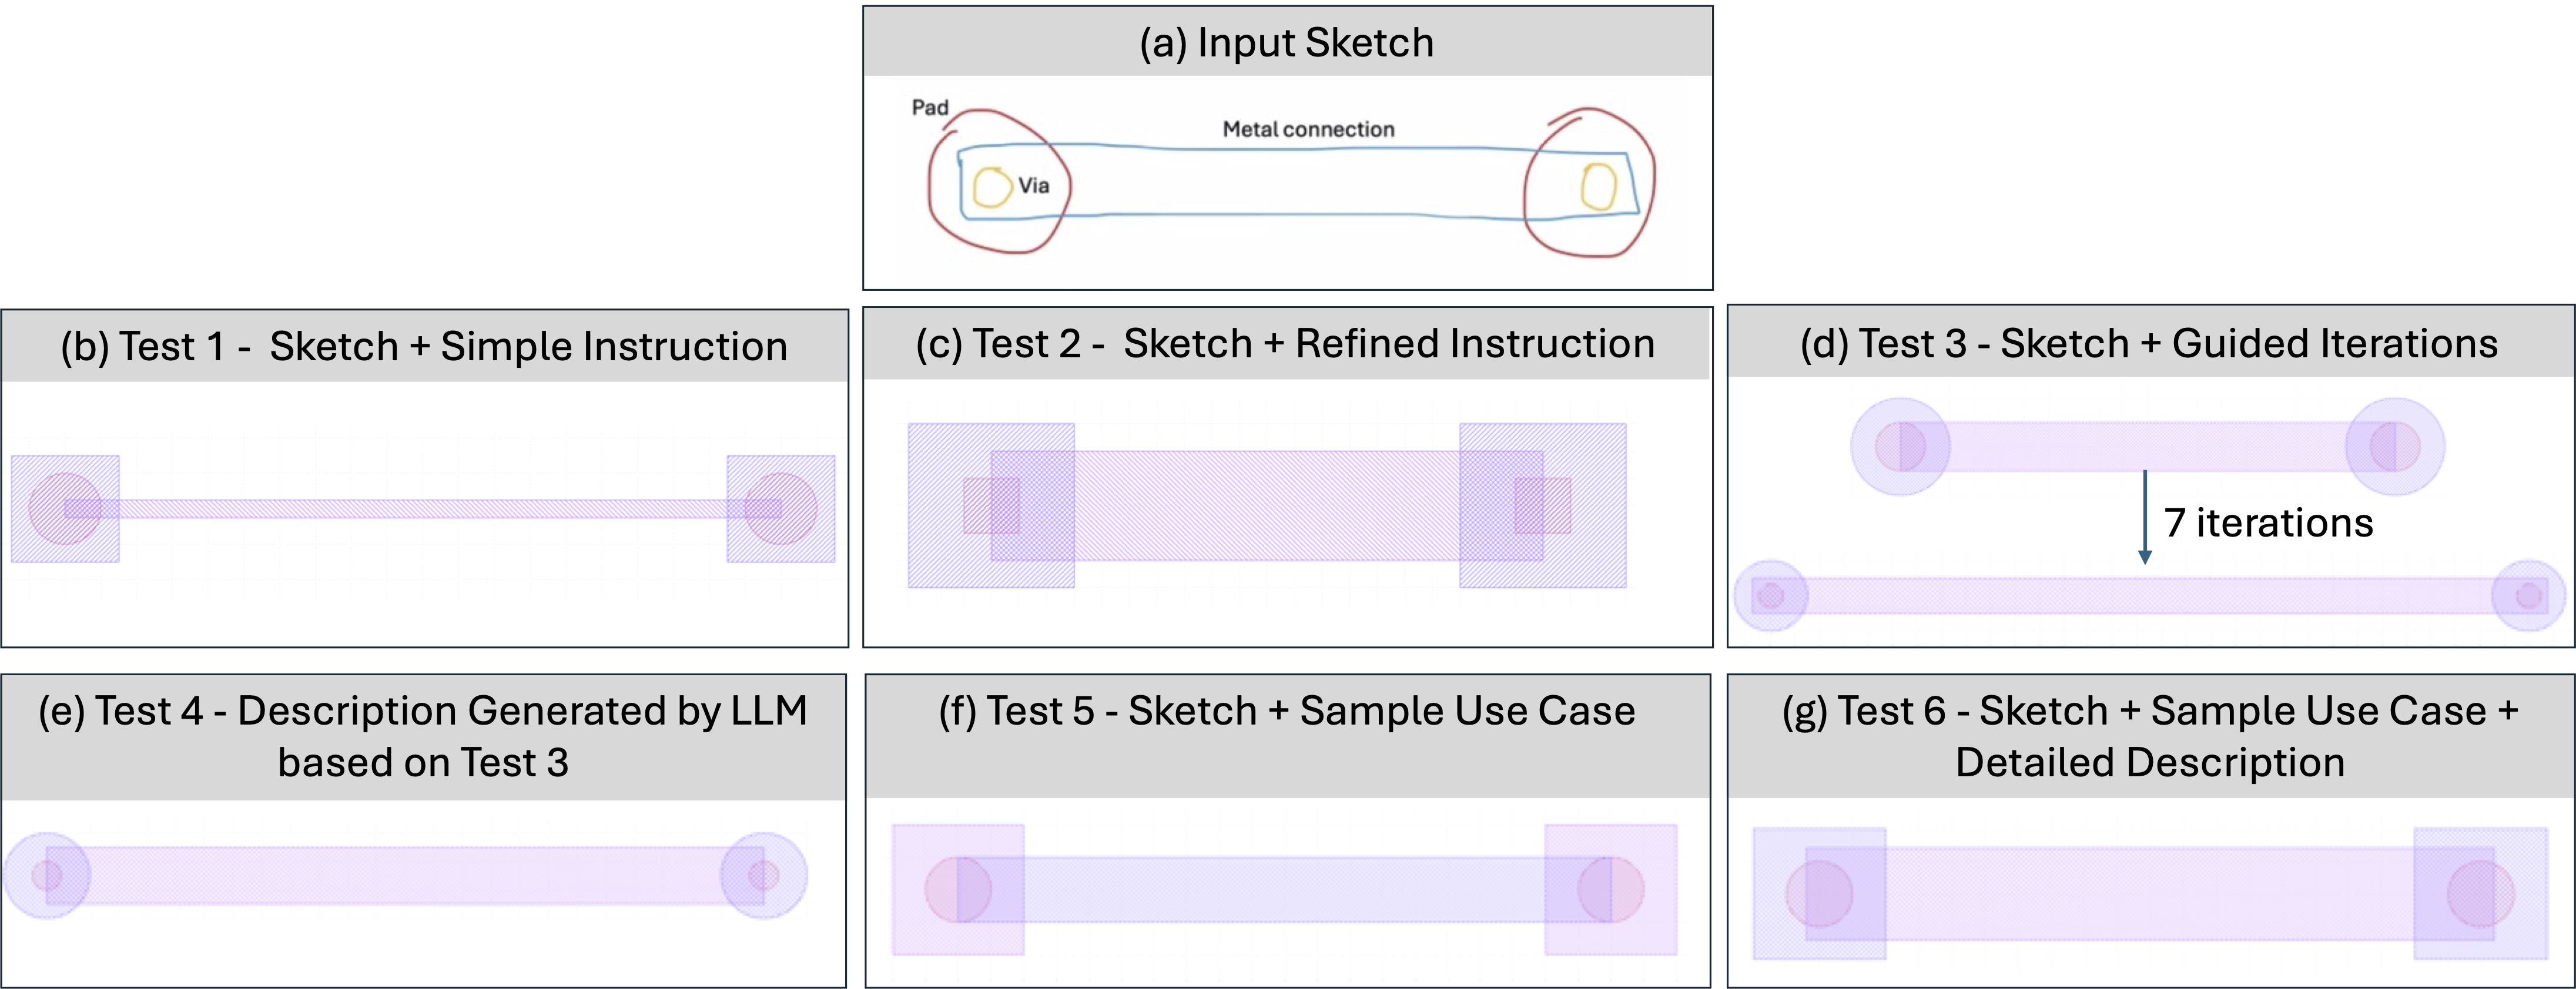
\includegraphics[width=1\linewidth]{Styles/Figure1_v3.png}
\caption{Sketch input and LLM-generated outputs for the via connection experiment. The sketch depicts a desired layout with two vias connected by a metal layer and circular pads on top. The outputs show the progression of the LLM's understanding and refinement of the layout based on iterative feedback and context provided by the user.}
\label{fig:via_experiment}
\end{figure}
In \textbf{Test 1}, we provided a basic sketch (Figure ~\ref{fig:via_experiment}(a)) along with a simple instructions to inform it each color represented a different layer. The LLM generated code based on this initial description; however, the output presented several issues, including incorrect dimensions for various elements and inaccurate layer relationships. \textbf{Test 2} involved refining the description, but limited improvement is observed. 

In \textbf{Test 3}, we gave a more detailed description accompanied by the original sketch. We proceeded with an iterative process, providing the LLM with feedback and screenshots of the GDSII file generated from its code. After seven iterations, the LLM successfully produced the correct layout. \textbf{Test 4} aimed to reproduce the best output from the previous test. We requested the LLM to create a detailed prompt based on the successful result from Test 3 and used this prompt to attempt to generate the correct output again. However, this approach proved ineffective, indicating that relying solely on an LLM-generated prompt to reproduce a layout was not reliable.

\textbf{Tests 5} and \textbf{6} gradually incorporated more context, such as 3D packaging, Through-Silicon Vias (TSVs), and other domain-specific requirements. However, adding domain knowledge and context did not improve the LLM's performance much, showcasing both its limitations and areas for potential improvement. Experienced engineers and researchers understand that connecting two vias requires using a metal layer wider than the diameter of the via. Moreover, vias should not be placed at the very ends of metal layers; some leeway is typically allowed between layers to accommodate potential misalignment.

The experiments demonstrate that LLMs currently lack the domain-specific knowledge possessed by experienced engineers, such as the need for wider metal connections between vias and leeway for misalignment. Despite incorporating more context and domain requirements in Tests 5 and 6, improvements were minimal, highlighting the gap in the LLM's understanding. While LLMs show potential in layout generation, they are not yet ready to replace human expertise, particularly in tasks demanding advanced semiconductor and microfluidics design knowledge. Future development should focus on embedding domain-specific rules and enhancing consistency and reproducibility.



\subsubsection{Lessons Learned}
The via connection experiment revealed several key findings:
\begin{itemize}
\item Clear, detailed, and context-rich input is essential for LLMs to generate accurate layout designs.
\item Iterative refinement and user feedback play a crucial role in guiding the LLM towards the desired output.
\item LLMs have limitations in understanding domain-specific requirements and constraints without explicit guidance.
\end{itemize}
\subsubsection{Potential Improvements and Future Work}
To enhance the sketch-to-design approach for via connections, we propose incorporating domain-specific knowledge and design rules into the LLM prompts. This can be achieved by providing a comprehensive set of guidelines and constraints as part of the input description. Additionally, future experiments should focus on validating the effectiveness of the improved approach and exploring its applicability to more complex via connection scenarios.

\subsection{Microfluidics Design}
% LLMs can guide researchers in estimating channel size based on fluid properties and dynamics
% Limitations: LLMs struggle with arithmetic calculations and may lack domain expertise

\subsection{Fiducial Marker Generation}
% LLMs perform well in generating fiducial markers on grids or arrays
% Advantages over commercial software: flexibility and potential other benefits

\subsection{General Discussion}
% The importance of spatial thinking, imagination, and understanding of physics for LLMs
% Need for providing use case requirements and expert knowledge as context to LLMs

\section{Conclusion and Future Work}
% Recap the main findings and insights
% Discuss the potential of LLMs in layout design and the challenges to overcome
% Outline future research directions:
%   - Dealing with more complicated designs
%   - Creating a benchmark to test LLM capabilities in layout design tasks
% Final thoughts on the role of LLMs as a "layout design copilot"
other domains, like mechanics, architecture

\printbibliography %Prints bibliography

\end{document}